\section{Phase 2: Personalized Multimodal Fusion}

In this phase, we analyse the data collected from the experiments mentioned in Section~\ref{sec:exp-phase2}, and apply decision-level fusion using weights that are calculated based on the MSE.

\subsection{Personalized Weights}

At the end of each task, we have facial and vocal predictions collected from the participant recordings. However, to properly evaluate how accurate those predictions are, we need a ground truth. Since emotion is a personal experience, we considered the self-reported emotional data provided by each participant as the ground truth. Participants reported which emotion they felt and how intense that emotion was. This information is used to calculate the personalized reliability of each modality for each person. The self-reported data is shown in the tables in Appendix~\ref{app:a}.

Then, Performed data cleaning by removing emotion labels that were outside the scope of our research. The remaining emotion labels were converted into arousal-valence values based on the mapping defined in Section~\ref{sec:emotion-mapping}. For comparison with self-reported values, we extracted the highest recorded emotion within each category from the system outputs. Participants were instructed to provide self-reported feedback by indicating the strongest emotion they felt during each task.

Subsequently, using the MSE-based weighting method described in Section~\ref{sec:exp-phase2-fusion}, modality-specific errors for each participant were calculated. These were then used to generate personalized fusion weights, as shown in Listing~\ref{lst:weights}. The resulting modality weights and corresponding MSE values are presented in Appendix~\ref{app:modality-mse}.

 


\subsection*{Analysis}  

A visual representation of the data presented in Appendix~\ref{app:modality-mse} is shown in Figure~\ref{fig:fusion-weights-visualization}, and the average fusion weights per emotion are illustrated in Figure~\ref{fig:average-fusion-weights}. Additionally, the distribution of the fusion weights across participants is displayed using a box plot in Figure~\ref{fig:weight-distribution}.

\begin{figure}[H]
    \centering
    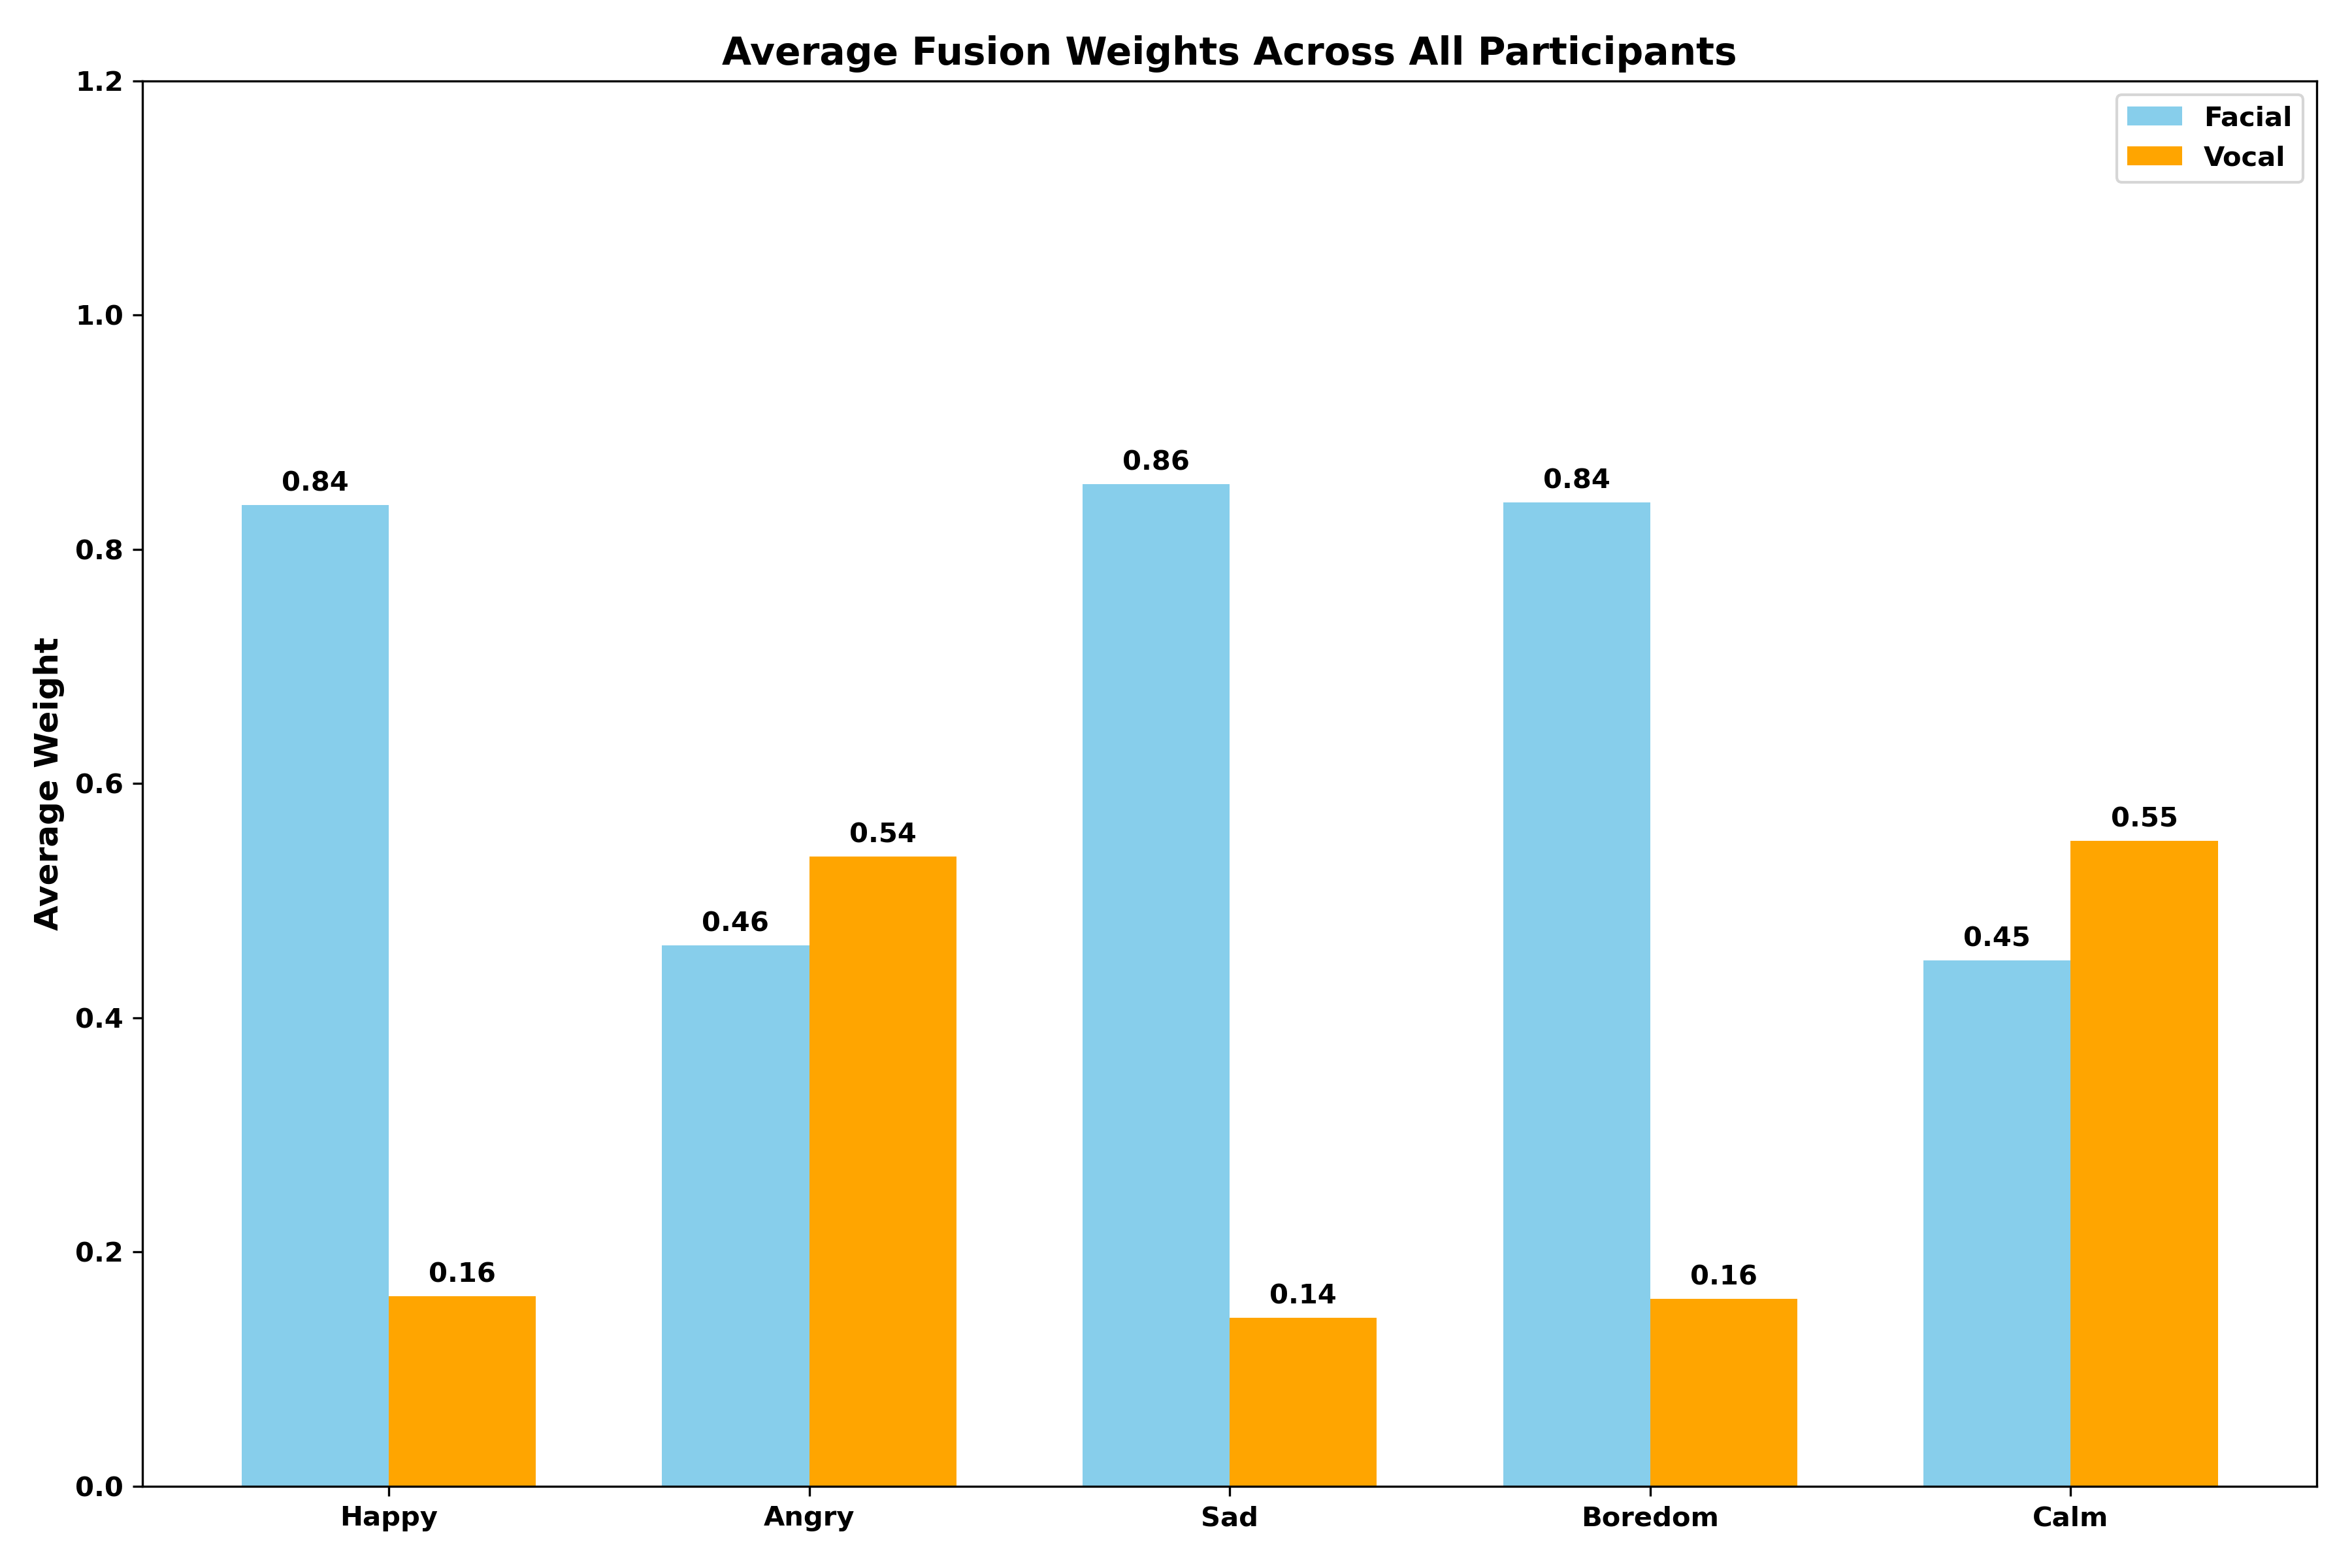
\includegraphics[width=1\textwidth]{img/chapter_04/weights/average_modified_fusion_weights.png}
    \caption{Average fusion weights per emotion category}
    \label{fig:average-fusion-weights}
\end{figure}

\begin{figure}[H]
    \centering
    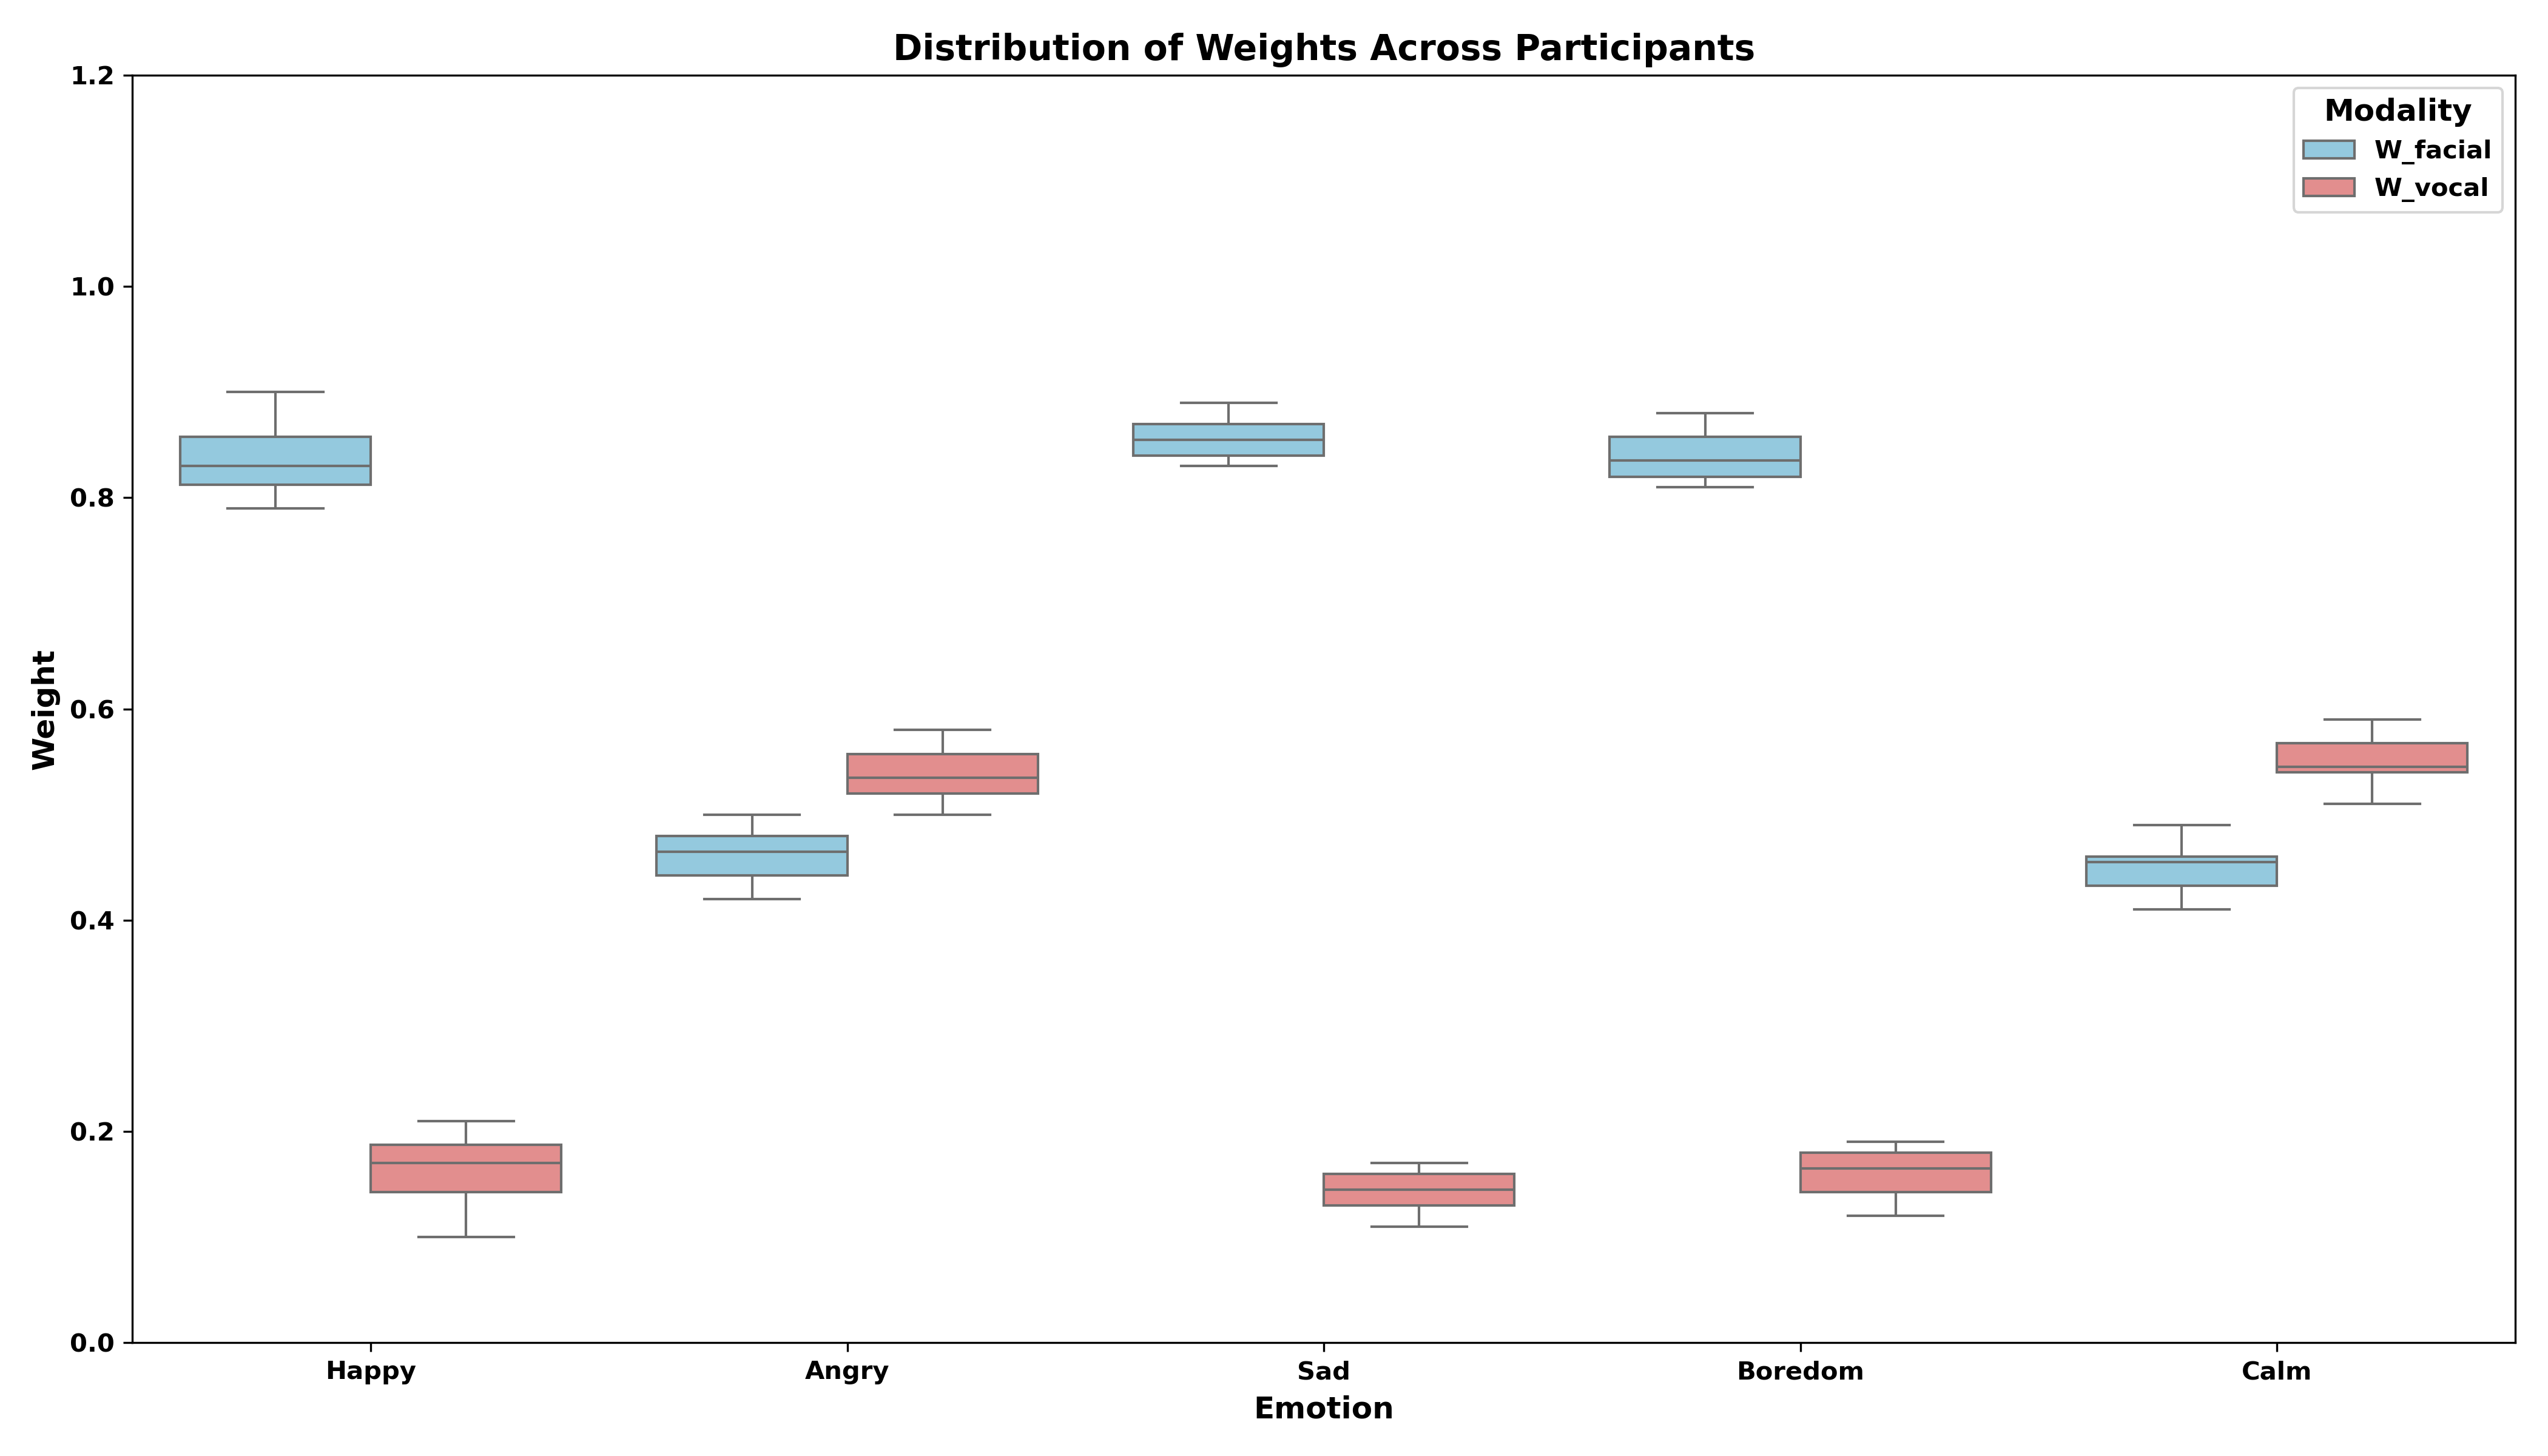
\includegraphics[width=.9\textwidth]{img/chapter_04/weights/weight_distribution_boxplot.png}
    \caption{Weight distribution boxplot across all participants}
    \label{fig:weight-distribution}
\end{figure}


\begin{figure}[H]
    \centering
    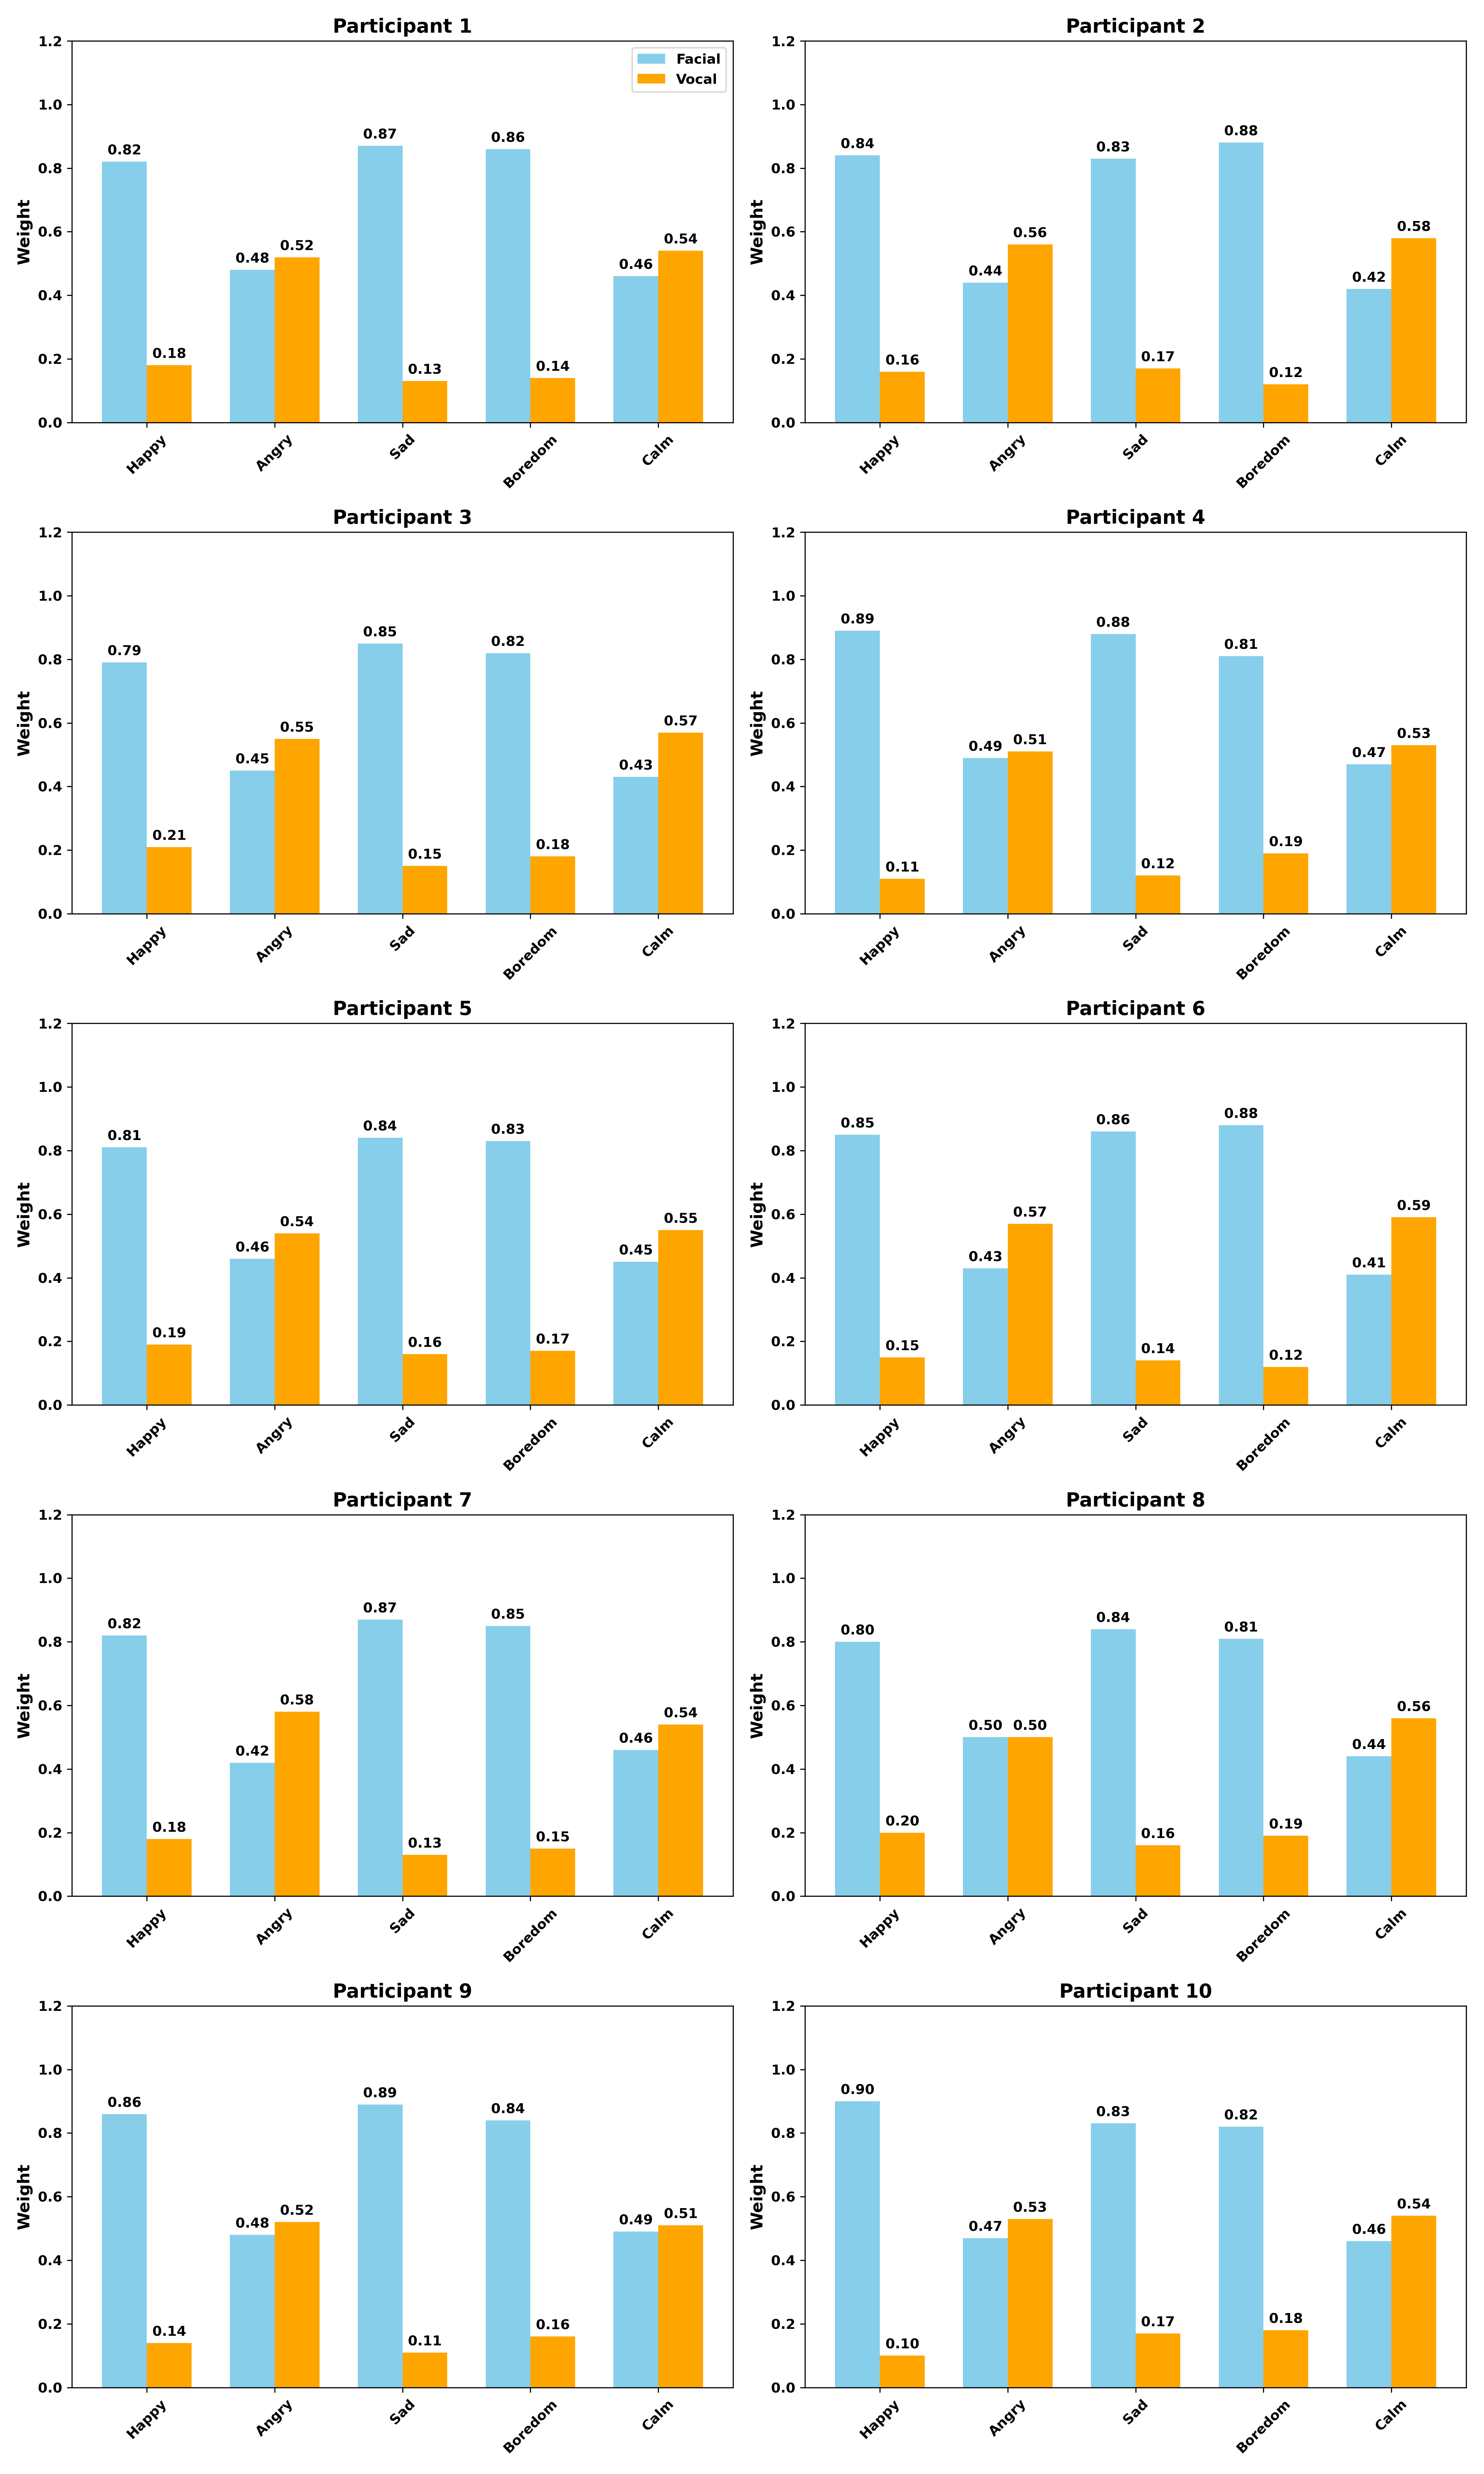
\includegraphics[width=1\textwidth]{img/chapter_04/weights/fusion_weights_visualization.png} 
    \caption{Fusion weight visualization for each participant}
    \label{fig:fusion-weights-visualization}
\end{figure}




The average fusion weights calculated for each emotion category are summarized below:

\begin{center}
\begin{tabular}{lcc}
\textbf{Emotion} & \textbf{W\textsubscript{facial}} & \textbf{W\textsubscript{vocal}} \\
\midrule
Angry   & 0.46 & 0.54 \\
Boredom & 0.84 & 0.16 \\
Calm    & 0.45 & 0.55 \\
Happy   & 0.84 & 0.16 \\
Sad     & 0.86 & 0.14 \\
\end{tabular}
\end{center}

From these weights, the dominant modality for each emotion was determined as follows:

\begin{center}
\begin{tabular}{lc}

\textbf{Emotion} & \textbf{Dominant Modality} \\
\midrule
Angry   & Vocal \\
Boredom & Facial \\
Calm    & Vocal \\
Happy   & Facial \\
Sad     & Facial \\

\end{tabular}
\end{center}

\textbf{Key Insights from Fusion Weight Analysis}

The analysis of fusion weights yields several interesting observations. Firstly, certain emotions such as Happy, Sad, and Boredom are predominantly recognized through facial expressions, with facial weights averaging over 0.84. On the other hand, Angry and Calm emotions appear to depend more on vocal cues, although the weights remain relatively balanced, indicating contributions from both modalities.

In terms of distribution, Happy and Sad emotions show the strongest modality preference, where the system clearly leans toward facial data. Conversely, the weights for Angry and Calm are more evenly distributed, suggesting that both modalities are essential for recognizing these emotions.

Furthermore, individual variations across participants show higher consistency in fusion weights for emotions like Happy, Sad, and Boredom. This implies that these emotions might have more universal expression patterns. However, for Angry and Calm, there is greater variation, pointing to the possibility that the expression of these emotions can differ significantly between individuals.
